\documentclass{article}
\usepackage[utf8]{inputenc}

\title{189G Term Project}
\author{Amber Graham, Sairamvinay Vijayaraghavan}
\date{12 December 2018}

\usepackage{natbib}
\usepackage{graphicx}

\begin{document}

\maketitle

\section{Problem A}
\subsection{Introduction}

In this problem, we investigated the accuracy of 4 different prediction methods on the given data set. The methods are described generally below:

\begin{itemize}
    \item k-nearest-neighbors (kNN): A method of prediction which finds the k most similar users to the user to be predicted for, and averages the k-users' ratings.
    \item non-negative matrix factorization (NMF): A method of prediction which splits a matrix of mostly unknown values into two completely known matrices (W and H). The product of WH is an entirely known matrix which can be used to predict the formerly unknown values.
    \item linear regression: A method of prediction which models a linear relationship
    \item method of moments: A statistical model for prediction which uses the expected values to derive the equations used to predict.
\end{itemize}

To evaluate the accuracy of these different methods we needed to test these models on the votes that were known. From the data set containing only known values, we could then split the data into a training and test set. The test set contained 1000 randomly selected user, bill, vote triplets and the train set contained all others. We then trained a model for each of the methods and predicted on the test set (pretending that we didn’t know the result).  Since the prediction resulted in decimal values, we rounded the prediction, and used this rounded value to calculate the accuracy of the prediction (number of correct predictions / total number of predictions.

We also calculated the mean absolute prediction error (MAPE) for the predictions, but found that this did not make sense for this particular data set since there are only two possibilities (0 for no and 1 for yes). The error was not as meaningful or intuitive as the PGEC. 

After the accuracies were calculated for each method, we compared the results. 

\subsection{Data Formatting}

We first needed to get the data into four columns in this order: member ID, bill ID, vote, and party so that we could use the prediction tools available in the rectools library which require this format. We gave each bill a numerical ID from 1 to 16. Then, we had to make each column numeric. This was simple for the user ID and bill ID, however we had to replace the “no” and “yes” values in the vote column with 0s and 1s and the “republican” or “democrat” values in the party column also with 0s and 1s.

\subsection{kNN best K analysis}



K Nearest Neighbor is one of the most fundamental prediction algorithms in recommender systems. We first had to determine which value of k (the number of nearest neighbors) would be the most optimal for this data set. We set k to various values (as shown below) and calculated the PGEC (accuracy) for each k.

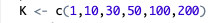
\includegraphics[]{krangeofvalues.png}

For kNN, we also looked at the difference in PGEC when covariates were included and not included. There was only one covariate in this case -- the political party of the congressmen. We obtained these results:

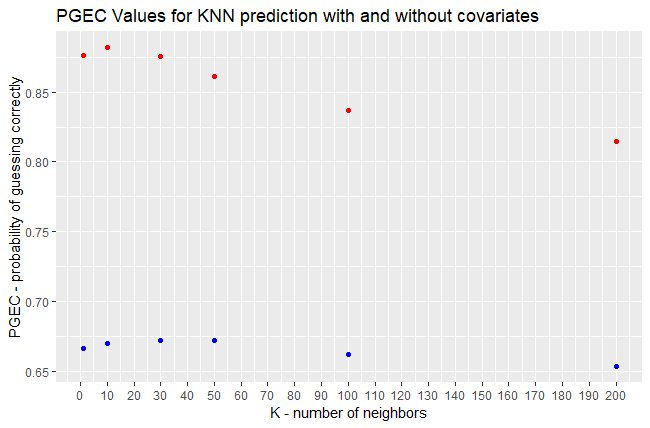
\includegraphics[scale = 0.7]{pgecknn.png}


The red dots indicate the predictions done including the covariates while the blue indicate the predictions performed without the covariates. From this graph we find that the prediction with covariates provide a much better prediction than the prediction without covariates.

You can see from this graph that the best PGEC we received for the kNN method was when k = 10. The PGEC is 0.87.


\subsection{NMF best r analysis}



Non-negative matrix factorization (NMF) is another fundamental method which is particularly useful because it offers some dimension reduction (the process of making the amount of data smaller and more manageable). This methods reduces the dataset of predictions into two simpler matrices of rank "r". Similar to kNN, we also needed to determine which r value would result in the highest PGEC for this dataset. The r values were as follows:

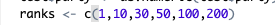
\includegraphics[]{rrangeofvalues.png}

Again, the PGEC was calculated when the covariate was included and when the covariate was not included. The following graph displays the PGEC calculation for each r value.

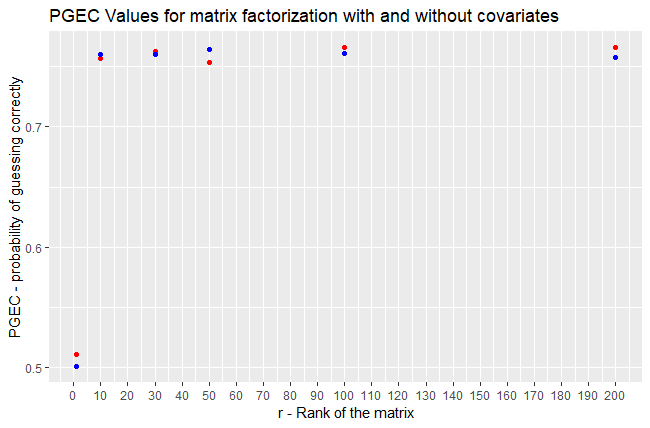
\includegraphics[scale = 0.7]{nmfpgec.png}

The red dots represent the prediction with the covariate and the blue dots represent the prediction without the covariate. The results again show that the prediction was slightly better with the covariates.

The highest PGEC was obtained when the rank was equal to 100 or 200 and with the covariate. This value is 0.766, which shows that nmf is an effective method of prediction for this dataset.


\subsection{Linear Regression}


This method is the full linear regression method which uses the concept of statistical models. We used the lm() method which creates the linear model for the train set and then predict.lm to predict the vote. To train the model, the votes were regressed against all other values, including the covariate (political party). We predicted against the test set as usual and obtained the following PGEC:

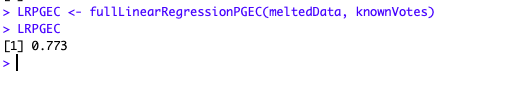
\includegraphics[scale = 0.7]{LMoutput.png}

The linear model resulted in an accuracy of 0.773. This shows that the linear model was indeed an effective measure of prediction for this dataset.

\subsection{Method of Moments}



The method of moments uses the concept of statistical models to predict. We used the rectools function trainMM() which computes all the latent factors for the train set. We also used the covariate (party affiliation) to train the method of moments model. We obtained the following results:

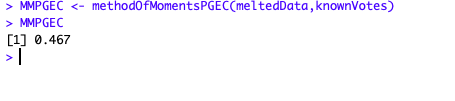
\includegraphics[scale = 0.7]{MMoutput.png}

This means that less than half of the predicted values were correct. Method of moments is not a reliable prediction method for this data set.

\subsection{Conclusion}


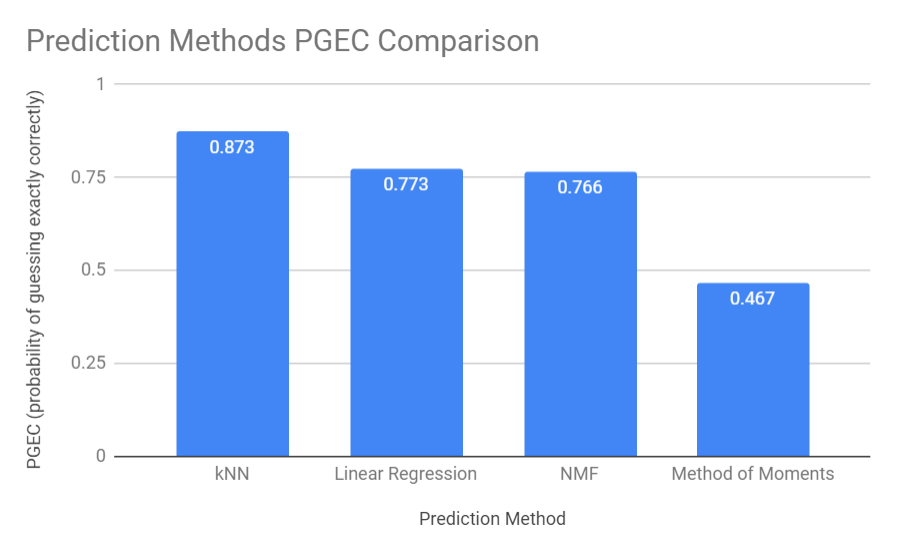
\includegraphics[scale = 0.4]{pgeccomparison.png}

Above you can see the comparison between the accuracies of the four different methods that we tested models with. Even though kNN seemed to have resulted in the highest PGEC, we decided to predict the missing votes in the data set with all four methods to see how similar the predictions were for each of the methods.

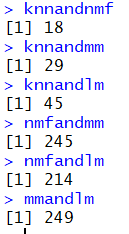
\includegraphics[scale = 0.6]{comparison.png}

The above shows the number of predictions that were the same for each of the methods. For example, the value of "knnandnmf" is the number of predictions that were the same between the knn method and nmf method -- they had 18 predictions that were the same for the missing data in the data set.

As you can see, the number of predictions that were the same for any method compared to kNN is very low. Even comparisons with the results for method of moments (which had the lowest PGEC) resulted in a higher count of same predictions. This made us very uncertain that our implementation of kNN was correct and that the extremely high PGEC that we found might be inaccurate. 

Therefore, we conclude that linear regression was the best method of prediction for this data set that we tested, and nmf follows close behind. 

\section{Problem B}

\subsection{Introduction}


In this problem, we explored the ability of sentiment analysis on verbal reviews to predict numerical ratings that user's gave for different drugs. We were provided with two data sets: the train data (to train the models with) and the test data (to test the models with). The files have 7 columns each which define: the drug name, the condition, the verbal review by the user, the user's rating for the given drug, and the "useful count" which is the number of users who found a review useful. 

To explore how well sentiment analysis works in determining a user's rating, we first had to use a sentiment analysis library on all of the reviews (in both the training and test set) to determine a numeric sentiment score. Then, we created models with the training set based off of the relationship between the sentiment scores and the user's ratings. Finally, we could predict user ratings from the sentiment scores in the test set and compare the results to the actual ratings in the test set. We used mean absolute prediction error (MAPE).

We also explored whether or not the other information provided in the data (drug type, condition, etc.) improved the MAPE for each method. 

Finally, we decided to do an experiment on filtering the reviews based off of the useful count. We noticed that sometimes reviews were not even written about the drug, and thus could have a negative affect on the overall MAPE. So, we thought that filtering out the reviews that people did not find useful might help improve the prediction. 

We used two different methods of prediction :
\begin{itemize}
    \item Linear Regression : This method forms a linear model on the train Data set and the model is then used to predict the ratings of the test set.
    \item Neural network: This method forms a neural network around the train data and then predict() method is called to predict on the neural network.
\end{itemize}

\subsection {Libraries Used}
\begin{itemize}
    \item Syuzhet: Used the get\_sentiment function on each of the verbal reviews to determine a numeric sentiment score
    \item DeepNet: Used the train.nn method to train a neural network
\end{itemize}

\subsection{Data Formatting}


We had a challenge when assigning a numeric value for almost all of the columns. Before formatting, only usefulCount and V1 was numeric. The drugName and the condition were just characters. These columns were converted to the factors data type when we read in the file in R and we had to then use the as.numeric() method to convert into numeric type. After these changes, only review was left which is a pure character string. We used sentiment analysis which provides a numeric score based on sentiments in a given character string. These scores were calculated for each of the reviews and since we wanted to retain these values in all of our predictions, we had created a new column called rev\_score which stores the sentiment rating of the review. This was performed for both the test and train sets.

\subsection{Linear Regression}
\subsubsection{Regression of the user rating against only the sentiment score}

 
 In this method, we predicted the ratings by training a linear model that regressed the users rating against only the sentiment score. This was done because we wanted to analyze the effectiveness of the sentiment analysis on the reviews alone and this was best achieved by eliminating all other covariates. We used only rev\_score column to train the linear model in this case. The resulting linear model created with the train data was used to predict the ratings in the test set. The mean absolute prediction error (MAPE) values was then calculated for each of the predicted ratings. The resulting MAPE is below: 

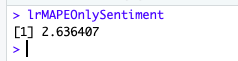
\includegraphics[scale = 0.8]{linSentOnly.png}

This result is the average absolute difference between the ratings predicted and the actual ratings. The average difference of 2.63 shows is a high MAPE considering the fact that user ratings are only between 1-10. Because this is an absolute value of the error, this means that the error is either (on average) 2.63 above the user's rating, or 2.63 below the user's actual rating. This is a very large range of error. Therefore, using the sentiment score alone to predict user ratings is not very effective for a linear model.

\subsubsection{Regression of the user rating against other covariates}

With this method, ratings were predicted using a linear model that regressed user ratings against all other covariates in this case to study the effect of the sentiment score with other information supporting it. The covariates used along side the rev\_score was the drug name, useful count and the condition. A similar process to the above linear regression was carried out and the MAPE was found as follows for this method:

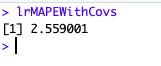
\includegraphics[scale = 0.8]{linCovsAll.png}

These results show that the MAPE was 2.559 which means that the difference between the predicted ratings and the true ratings on average is 2.559. This MAPE shows that the linear regression against all the other covariates including the sentiment score provides a slightly more accurate prediction compared to the prediction with only the rev\_score as the single covariate of prediction.

\subsection {Neural Networks}
\subsubsection{Training a Neural Network to determine user rating with only the sentiment score}
With this method, we trained a neural network using the library "DeepNet." Similar to the linear regression method, we wanted to first train the network with only the sentiment score so we could analyze the ability of the sentiment score alone to accurately predict the user rating. 

The resulting MAPE was 2.733.

\subsubsection{Training a Neural Network to determine user rating with other covariates}

With this method, we again trained a neural network using the libary "DeepNet." Instead, this time we included some covariates. We were not able to include the date covariate and the verbal review of course because these could not be expressed as numerical values. 

The resulting MAPE was 2.901.

This MAPE is worse than when covariates were not involved. Neural networks are very prone to overfitting, which is when the model works so well on a given train set that it does not perform as well when working with other data. We believe that is what happened here -- adding in the covariates resulted in a a model that was too good, which resulted in overfitting and a worse MAPE on the test set.


\subsection{Filtering Data based off of a high "useful count" to decrease MAPE}

Because the resulting MAPES from our previous methods were so high, we decided to try and filter the data based off of the "useful count" which is the number of users that find a given rating useful. We used useful count because we thought it might be a good measure of the relevance of a review. If a review is actually useful (i.e. maybe they actually talked about what they liked or disliked about the drug they are reviewing), we thought that the sentiment score for that review might correlate better with the user's rating.

To implement this, we filtered the test data to only include rows where the useful count was greater than a given threshold. We also calculated the mean of all the useful counts and included this value in our test (we assume that if the usefulCount for any review is the average of the usefulCount, then we picked the above average relevant reviews). We tested our idea on each of the four methods that we described previously (linear model with and without covariates, neural network with and without covariates). Here's the range of the values of the useful counts that we tested:

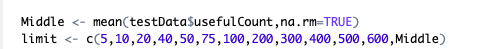
\includegraphics[]{usefulCountrange.png}


\subsection{Linear Regression with Filtered Data}
\subsubsection{Regression of the user rating against only the sentiment score}

Similar to the linear regression discussed in the previous sections, we trained a model using the entire train set. We predicted using a filtered test data set which was updated each time for each different threshold on the useful count. The regression was performed only against sentiment score which again helped us visualize the effect of the rev\_score alone on the rating. The MAPE was calculated for each of the different test sets with different thresholds, and the results are displayed in the graph below:

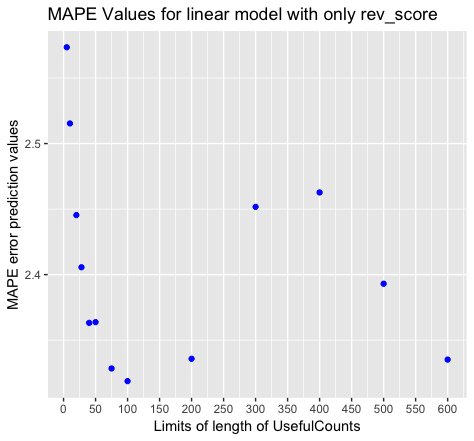
\includegraphics[scale = 0.6]{LRS_filter.png}


These results show that the MAPE values start to generally decrease when the threshold value increases and it slightly increases as the threshold increases from 300 onwards. This is because the number of rows to predict drastically decrease as the limit increases and hence the predictions start to become more erroneous.

The best MAPE for this method is 2.3187 and was achieved with a useful count threshold of 100 (the test set only included ratings that had a useful count greater than 100). 



\subsubsection{Regression of the user rating against other covariates}

This time, we performed regression on the similar filtered test data set but we regressed against all the other covariates. We obtained the following results:

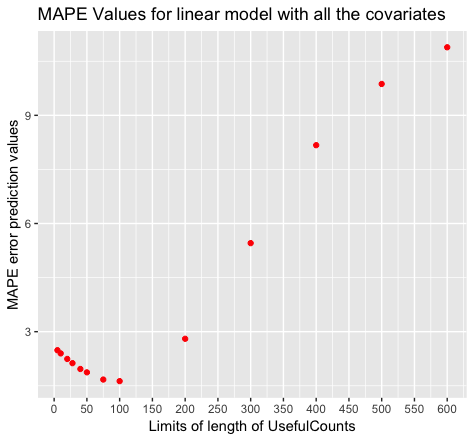
\includegraphics[scale = 0.6]{LRC_filter.png}

Because the size of the data set to predict on shrinks as the threshold increases, there's an unusually higher MAPE compared to the previous thresholds. 

With this method, we achieved the best MAPE when the threshold was 100 -- a value of 1.63.

The graph of distribution across all thresholds is as follows: 


\subsection {Neural Networks with Filtered Data}
\subsubsection{Training a Neural Network to determine user rating with only the sentiment score}
    
    Next we performed the same useful count analysis on the neural network model. We first performed the analysis on a neural network model that was created based off of the relationship between the ratings and only sentiment score in the train data. The results for each threshold are shown below:
  
   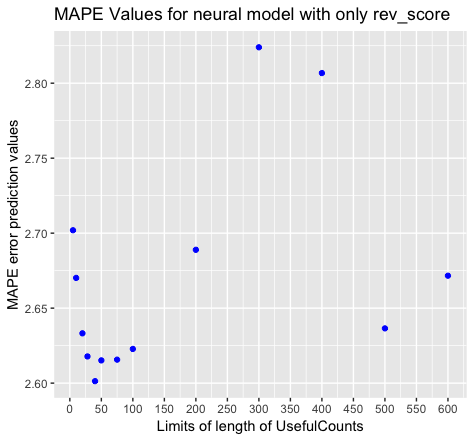
\includegraphics[scale = 0.8]{DNS_filter.png}  
 
 This results are very different from the results that we obtained from the linear regression model. In this case, all of the MAPE values are within the range 2.6 to 2.8 approximately. Before, the values were in a much larger range. It seems as if the useful count thresholds on a neural network have an overal positive affect on the MAPE (these are still lower than the results without the useful count filtering). However, there is not nearly as much variance between the individual thresholds.
 
 Below is a graph of the results: 
 

 
\subsubsection{Training a Neural Network to determine user rating with other covariates}

Next we also checked how the useful count filtering worked for neural networks when covariates were involved. The results are below:

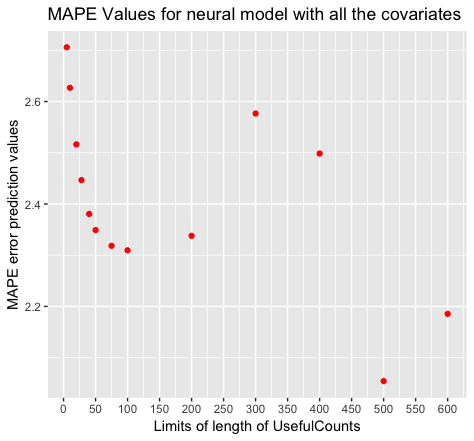
\includegraphics[scale = 0.6]{DNC_filter.png}

The lowest MAPE obtained here is approximately 2.05, however, this was obtained when the threshold was at 500, which means that it the test set had very little data in it. However, if we consider the data before the threshold of 300, the lowest MAPE was 2.31, which is still lower than the previous method. It is interesting to note that this might have eliminated the overfitting problem -- the model with more covariates now performs better than the model without covariates. Overall, the variance between the two results is not very high anyways, so this may be because we are just looking at less data here.

\subsection{Results}

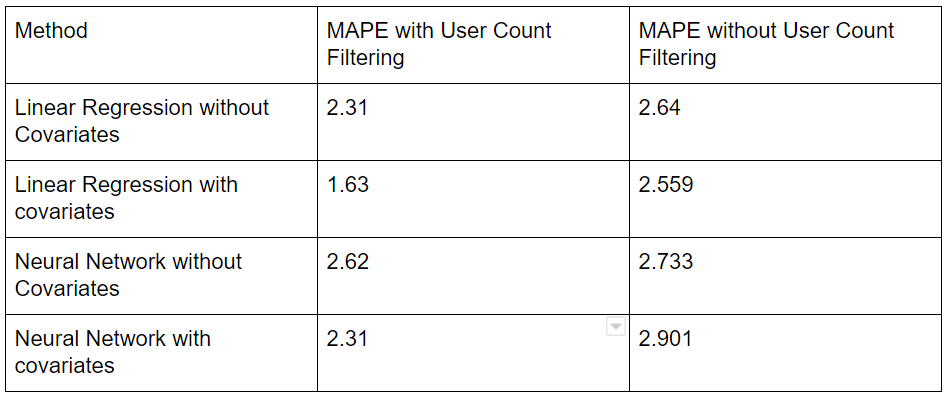
\includegraphics[scale = 0.8]{problemBresults.png}
The results for the best MAPEs for each of our tests are shown above. 
This chart shows two important things. The first is that the user count filtering proved to improve the MAPE for every method we tested. The second is that linear regression seemed to perform better than the neural network in all instances.

\subsection{Conclusion}

The best MAPE that we received for this experiment was when we used useful count filtering with the linear regression model with covariates. This value was 1.63, which is unfortunately still high. This could allow someone to maybe get a general idea of how a user rated based off of their verbal reviews, but it still would not be very accurate. 

We found that it would be very difficult to determine the rating based off of sentiment analysis of reviews. This is because reviews might not have anything to do with the drug at all, or may even be non-sensical. Topic modeling or some other form of advanced natural language processing would have to be used in order to get more accurate results.

\section{Team Member Participation}
Sairamvinay Vijayaraghavan
\begin{itemize}
  \item Problem A 
    \begin{itemize}
        \item kNN implementation (Worked on it together)
        \item NMF implementation
    \end{itemize}
  \item Problem B
    \begin{itemize}
        \item Data formatting
        \item Finding a good sentiment analysis library
        \item Useful Count filtering implementation
        \item Linear regression implementation
    \end{itemize}
\end{itemize}
Amber Graham
\begin{itemize}
  \item Problem A 
    \begin{itemize}
        \item kNN implementation (Worked on it together)
        \item Full Linear Regression implementation
        \item Method of Moments implementation
        \item Prediction of missing values for each prediction method
        \item Data formatting
        
    \end{itemize}
  \item Problem B
    \begin{itemize}
        \item Finding a good neural network library
        \item Neural Network implementation
    \end{itemize}
\end{itemize}

\section{Code}

\item ProblemA:

    \begin{itemize}
        \item getMeltedData(): Reads in the data file and does the data formatting. Returns the data frame containing the converted userIDs, covariates and ratings as 1 or 0.
        \item getKnownVotes(meltedData): returns the data set with all the votes that are not ? 
        \item getMissingData(meltedData): returns the data set with all the votes that are ?
        \item knnBestKAnalysis(meltedData,knownVotes): returns graph of both PGEC and MAPE spread accross various k in knn.
        \item nmf\_analysis(meltedData,knownVotes): returns graph of both PGEC and MAPE spread accross various ranks in nmf.
        \item knn\_bestMAPE(meltedData, knownVotes): returns the dataframe with k and respective MAPE
        \item knn\_bestPGEC(meltedData, knownVotes): returns the dataframe with k and respective PGEC
        \item nmf\_bestMAPE(meltedData,knownVotes):returns the dataframe with k and respective MAPE for nmf
        \item nmf\_bestPGEC(meltedData,knownVotes) :returns the dataframe with k and respective PGEC for nmf
        \item fullLinearRegressionMAPE(meltedData, knownVotes): returns the MAPE for a linear model with covariates
        \item fullLinearRegressionPGEC(meltedData, knownVotes): returns the PGEC for linear model on melted data
        \item methodOfMomentsMAPE(meltedData, knownVotes): returns the MAPE for MethodofMoments
        \item methodOfMomentsPGEC(meltedData, knownVotes): returns the PGEC for MethodofMoments
        \item knnPredictUnknownVotes(meltedData): returns a vector of all of the predictions for the unknown values using kNN
        \item fullLinearRegressionPredictUnknowns(meltedData): returns a vector of all of the predictions for the unknown values using a linear model
        \item nmfpredictunknowns(meltedData) returns a vector of all of the predictions for unknown values using the nmf method

    \end{itemize}
\item ProblemB:
   \begin{itemize}
    \item linearRegressionMAPE(trainData,testData,onlySentiment): This function creates a linear regression model from the trainData and predicts with the testData. If onlySentiment is true, the model will only regress against the sentiment score. Otherwise, it will regress against all covariates. The function returns the MAPE.
    
    \item deepnetMAPE(trainData,testData,onlySentiment): The function which does neural network prediction on the testData using the trainData. onlySentiment is used for only prediction with sentiment score alone. Returns the MAPE.
    
    \item useFulCountPlay(trainData,testData): The functions does the filtering of data using usefulCount as a threshold for filtering data and returns the list of five elements: limits (thresholds), MAPEs of linear regression with covariates, MAPEs of linear regression without covariates, MAPEs of neural network with covariates,MAPEs of neural network with covariates.
    
    
    
   
   
   
   \end{itemize}

\end{document}
